\section{Adaptive Estimation \label{sec:sequential}}
The first main results of this paper, as described in Theorem~\ref{thm:adpative_lower_bound} below, states that the ARE of any adaptive estimator cannot be larger than $\eta(0)\sigma^2$, which is the ARE of the median of the sample $X_1,\ldots,X_n$. We also provide a particular adaptive estimation scheme that attains this maximal efficiency. %Finally, in Theorem~\ref{thm:opt_one_step}, we provide an adaptive estimation scheme that is one-step optimal in the sense that at each step $i$, the chosen message $B_i$  minimizes the MSE given $X_i$ and the previous $i-1$ messages. %Numerical simulations for the case of $f(x)$ the normal density function shows that the ARE of the estimator described by this scheme is $\eta(0)\sigma^2$. 

\subsection{Limited efficiency in the adaptive setting}
Our first result asserts that the ARE of any adaptive encoding and estimation scheme is bounded from above by $\eta(0)\sigma^2$. %This result follows from the following theorem:
\begin{thm}[maximal relative effeciency] \label{thm:adpative_lower_bound}
Let ${\theta}_n$ be any estimator of $\theta$ in the adaptive setting of Figure~\ref{fig:setup}-(ii). Assumes that $\pi(\theta)$ converges to zero at the endpoints of the interval $\Theta$. Then
\[
n\mathbb E\left[ (\theta-{\theta}_n)^2 \right] \geq   \frac{n}{ 4f^2(0) n + I_0},
\]
where 
\[
I_0 = \mathbb E \left( \frac{d}{d\theta} \log \pi (\theta) \right)^2
\]
is the Fisher information with respect to a location model in $\theta$. 
\end{thm}

\subsubsection*{Proof}
%We first bound from above the Fisher information of any set of $n$ one-bit messages with respect to $\theta$. The result then follows using the van-Trees inequality which bounds from below the risk of any estimator of $\theta$ by the inverse of the expected value of the aforementioned Fisher information plus $I_0$. The details are in
See Appendix~\ref{proof:thm:adpative_lower_bound}.\par

Theorem~\ref{thm:adpative_lower_bound} implies that any estimator ${\theta}_n$ from any adaptive encoding scheme satisfies
\[
n\mathbb E\left[ (\theta-\theta_n)^2 \right] \geq  \frac{1}{4f^2(0)}+O(n^{-1}),
\]
and 
\[
\ARE({\theta}_n) \leq 4f^2(0)\sigma^2 = \eta(0)\sigma^2.
\]
It is possible to extend Theorem~\ref{thm:adpative_lower_bound} to any other loss functions using a more subtle version of the Van Tress inequality provided in \cite{efroimovich1980information}. See also \cite{DBLP:journals/corr/abs-1902-08582}. \par
%
Next, we provide an adaptive encoding and estimation scheme that attains the maximal ARE of $\eta(0)\sigma^2$. 

\subsection{Asymptotically optimal estimator}
Let $\left\{ \gamma_n \right\}_{n\in \mathbb N}$ be a strictly positive sequence. Consider the following estimator ${\theta}_n$ for $\theta$:  
\begin{equation}
\label{eq:sgd_alg}
\theta_n = \theta_{n-1} +  \gamma_n B_n, \quad n = 1,2,\ldots,
\end{equation}
where 
\begin{equation}
B_n = B_n (X_n,\theta_{n-1}) =\sgn (X_n - \theta_{n-1}).
\end{equation}
Define the $n$th step estimation as
\begin{equation} \label{eq:sgd_est}
\bar{\theta}_n =  \frac{1}{n} \sum_{i=1}^n  \theta_i. 
\end{equation}

We have the following results:
\begin{thm} \label{thm:sgd}
Consider the sequence $\left\{\bar{\theta}_n \right\}_{n\in \mathbb N}$ defined by \eqref{eq:sgd_est}. 
\begin{enumerate}
\item[(i)] Assume that $\left\{ \gamma_n \right\}_{n\in \mathbb N}$ satisfies
\begin{equation} \label{eq:conditions1}
\begin{cases}
\frac{\gamma_n - \gamma_{n+1}}{\gamma_n} = o(\gamma_n), &  \\
\sum_{n=1}^\infty \frac{\gamma_n^{(1+\lambda)/2}} {\sqrt{n}} < \infty, & 
\mathrm{for~some~}0< \lambda \leq 1
\end{cases}
\end{equation}
(e.g., $\gamma_n = n^{-\beta}$ for $\beta \in (0,1)$). Then
\[
\sqrt{n}\left( \bar{\theta}_n - \theta\right) \overset{d}{\to} \Ncal\left(0,\frac{1}{\eta(0)}\right).
\]
%
%
\item [(ii)] Assume in addition that $f(x)$ is continuously differentiable with a finite location Fisher information, namely
\[
I_\theta = \int_{\mathbb R} \left( \frac{f'(x)}{f(x)}  \right)^2 f(x) dx < \infty.
\]
%(or that $f(x-\theta)$ is differentiable in quadratic mean).  
Then for any bounded, symmetric, and quasi-convex function $L$, 
\begin{align} 
& \liminf_{c \to \infty} \liminf_{n \to \infty} \sup_{\tau\,:\,|\theta-\tau| \leq \frac{c}{\sqrt{n} }}  \mathbb E \left[ L\left( \sqrt{n}(\bar{\theta}_{n} - \tau) \right) \right] \nonumber 
\\
& \qquad \qquad \qquad \qquad = \mathbb E \left[ L (Z/\sqrt{\eta(0)}) \right], \label{eq:attaining_LAM}
\end{align}
where $Z \sim \Ncal(0,1)$. 
%
%
\item[(iii)] Assume that, in addition to \eqref{eq:conditions1}, $\left\{ \gamma_n \right\}_{n\in \mathbb N}$ satisfies
\begin{equation} \label{eq:conditions2}
\begin{cases}
\gamma_n = o(n^{-2/3}), &  \\
\sum_{n=1}^\infty \gamma_n = \infty.  & \\
\end{cases}
\end{equation}
(e.g., $\gamma_n = n^{-\beta}$ with $\beta \in (2/3,1)$). Then
\[
 \ex{\left( \bar{\theta}_n - \theta \right)^2} = \frac{1}{n\eta(0)} + o(n^{-1}). 
\]
\end{enumerate}
\end{thm}

\subsubsection*{Proof}
See Appendix~\ref{proof:thm:sgd}. \par

Theorem~\ref{thm:sgd} implies that the estimator ${\theta}_n$ defined by \eqref{eq:sgd_est} and \eqref{eq:sgd_alg} attains the maximal ARE, as established by Theorem~\ref{thm:adpative_lower_bound}. %Furthermore, it is locally minimax in the sense that it attains the minimal MSE for all local alternatives of $\theta$. 
%
The update step \eqref{eq:sgd_alg} can be seen as a gradient descent step for the function $x\to |x|$ at the point $x=X_n - \theta_{n-1}$. Consequently, the procedure above is known as averaged stochastic gradient descent for minimizing $x \to |x|$ given the data $X_1,\ldots,X_n$. The minimal value of this optimization is the sample median, and Theorem~\ref{thm:sgd} provides conditions for the sequence of gradient steps so that the algorithm converges to this minimum. In particular, parts (i) and (ii) of Theorem~\ref{thm:sgd} provides conditions under which $\bar{\theta}$ is asymptotically normal and local asymptotically minimax, in the sense that it attains the local asymptotic minimax bound \cite{van2000asymptotic}. Part (iii) provides an additional condition under which $\bar{\theta}$ also converges in its second moment. 
 \par
%Note that $\theta_0$ is not explicitly defined in equation \eqref{eq:sgd_est}. A reasonable initialization for $\theta_0$ is $\theta_0 = \mathbb E [\theta]$, although Theorem~\ref{thm:sgd} implies that the asymptotic behavior of the estimator is indifferent to this initialization. Thus, the optimal efficiency is attained regardless of the prior distribution on $\theta$ or the radius of the parameter space $\Theta$.  \\
In the encoding and estimating procedure \eqref{eq:sgd_alg} and \eqref{eq:sgd_est}, each one-bit message $B_n$ depends on its private sample as well as the current gradient descent estimate $\theta_{n-1}$. In this sense, each encoder in this algorithm interacts with previous one by using the current estimate.
%
As we explain next, 
it is possible to obtain the optimal efficiency of $\eta(0)\sigma^2$ with only one round of interactions among the encoders. 


\begin{figure}
\begin{center}
\begin{tikzpicture}[node distance=2cm,auto]
  \node at (0,0) (source) {$X_1$} ;
  \node[int1, right of = source, node distance = 1.2cm] (enc1) {$\enc$};  
\draw[->,line width = 2pt] (source) -- (enc1); 

% \node[below of = source, node distance = 1cm] (source2) {$X_2$};
%\node[int1, right of = source2, node distance = 1.2cm] (enc2) {Enc};  
%\draw[->,line width = 2pt] (source2) -- (enc2); 

\node[below of = source, node distance = 1.7cm] (source3) {$X_{n_1}$};
\node[int1, right of = source3, node distance = 1.2cm] (enc3) {$\enc$};  

\draw[->,line width = 2pt] (source3) -- (enc3); 

\node[below of = source, node distance = 0.5cm] {$\vdots$};

\node[int1, right of = enc3, node distance = 2.1cm ] (est) {$\est_1$};

\draw[->,line width = 2pt] (enc1) -| node[above, xshift = -1cm] (mes1) {$B_1$} (est);   

%\draw[->,line width = 2pt] (enc2) -| node[above, xshift = -1cm] (mes2) {$B_2$} (est);   

\draw[->,line width = 2pt] (enc3) -- node[above, xshift = 0cm]  {$B_{n_1}$} (est);   

\node[below right = 0.75 and 1.5 of source3] (sourceB) {$X_{n_1 +1}$} ;
\node[int1, right of = sourceB, node distance = 1.7cm] (enc1B) {$\enc$};  
\draw[->,line width = 2pt] (sourceB) -- (enc1B); 

\node[below of = sourceB, node distance = 1.7cm] (source3B) {$X_n$};
\node[int1, right of = source3B, node distance = 1.7cm] (enc3B) {$\enc$};  
\draw[->,line width = 2pt] (source3B) -- (enc3B); 
\node[below of = sourceB, node distance = 0.4cm] {$\vdots$};

\node[int1, right of = enc3B, node distance = 2.1cm ] (estB) {$\est_2$};

\draw[->,line width = 2pt] (enc1B) -| node[above, xshift = -0.5cm] {$B_{n_1+1}$} (estB);
\draw[->,line width = 2pt] (enc3B) -- node[above] {$B_n$} (estB);

\draw[->,line width = 1pt] (est.east) node[above, xshift  =0.5cm] {${\theta}_{n_1}$} -| (enc1B.north);

%\draw[->,line width = 1pt] (enc1B) -- (enc3B);

\draw[->,line width = 0.5pt] (est.east) -| +(1.3,-0.5) -- +(1.3,-2.5) -| (enc3B.north);

%\draw[->,line width = 1pt] (enc1B)  -- node[right] {${\theta}_{n_1}$} (enc3B);

\draw[->,line width = 0.5pt] (estB) -- +(0.8,0) node[right] {${\theta}_n$};
\node[below of = enc1B, node distance = 0.5cm] {$\vdots$};

\end{tikzpicture}
\end{center}
\caption{Distributed encoding with a single interaction: The estimation obtained from the first $n_1$ bits in a distributed manner is to obtain another $n-n_1$ bits in a distributed manner. 
\label{fig:one_round}
}
\end{figure}

\subsection{Maximal Efficiency using One Round of Threshold Adaptation}
In Section~\ref{sec:preliminary} we considered an estimator that is based on binary messages of the form 
\[
B_i = \mathbf 1_{X_i > \theta_0},\qquad i=1,\ldots,n,
\]
and deduced that it is asymptotically normal with variance $1/\eta(\theta-\theta_0)$.
%
We now show that a similar encoding leads to an asymptotically normal estimator attaining the lower variance bound $1/\eta(0)$, provided we allow to  update the threshold value $\theta_0$ based on previously observed bits at least once. 
%
In this procedure we separate the sample into two disjoint sets: $X_1,\ldots,X_{n_1}$ and $X_{n_1+1},\ldots,X_n$ for some $n_1 < n$.
We first use the estimator \eqref{eq:estimator_naive} to obtain an estimate ${\theta}_{n_1}$ based on $B_1,\ldots,B_{n_1}$, and then use ${\theta}_{n_1}$ as the new threshold value to obtain messages $B_{n_1+1}, \ldots, B_n$. Figure~\ref{fig:one_round} illustrates a diagram of this procedure. 
%
The specific encoding and estimation scheme, as well as its asymptotic performance, are given by the following theorem:
\begin{thm}
For $i=1,\ldots,n$ set
\[
B_i = \begin{cases}
 \mathbf 1_{X_i \geq \theta_0} & i = 1,\ldots,n_1, \\
 \mathbf 1_{X_i \geq {\theta}_{n_1} }& i={n_1+1,\ldots,n},
\end{cases}
\]
where $n = n_1+ n_2$ and 
\[
{\theta}_{n_1} \triangleq \theta_0 + F^{-1}\left(
\frac{1}{n_1} \sum_{i=1}^{n_1} B_i 
 \right).
\] 
Let 
\[
{\theta}_{n_2}  = {\theta}_{n_1} +  F^{-1} \left( \frac{1}{n_2} \sum_{i=n_1+1}^{n_2} B_i \right)
\]
and assume that $n_1(n) \rightarrow \infty$ and $n_1(n)/n \rightarrow 0$. Then:
\begin{align*}
 \sqrt{n} \left( {\theta}_{n_2} - \theta  \right) \overset{d}{\longrightarrow}  \Ncal\left( 0, 1/\eta(0) \right).
\end{align*}
\end{thm}
%
%
\begin{proof}
For $t\in \mathbb R$, set
\[
p_{n_2}(t) \triangleq \frac{1}{n_2} \sum_{i=n_1+1}^{n} \mathbf 1_{X_i \geq t}. 
\]
From the central limit theorem
\begin{align*}
& \sqrt{n} \left( p_{n_2}(t) - F( \theta - t) \right)  = \sqrt{\frac{n}{n_2}} \sqrt{n_2} \left(  p_{n_2}(t) - F(\theta - t) \right) \\
& \overset{d}{\rightarrow} \Ncal\left( 0, V(t) \right),
\end{align*}
where
\[
V(t) \triangleq F(\theta - t) F \left( t - \theta\right). 
\]
Applying the delta method to $p_{n_2}(t)$ with $g(x) = F^{-1}(x)$ implies
\begin{align*}
& \sqrt{n} \left( t + F^{-1}(\hat{p}_{n_2}(t)) - \theta \right) \\
&= \sqrt{n} \left( g(\hat{p}_{n_2}(t)) - g \left(F(\theta-t) \right)  \right) \\
& \overset{d}{\to} \Ncal\left(0, 
1/\eta(\theta-t) \right).
\end{align*}
%where this convergence is uniform in $t$ since all moments of $F^{-1}(\hat{p}_{n_2})$ exists. 
On the other hand, by the law of large numbers,
\[
p_{n_1} \triangleq \frac{1}{n_1} \sum_{i=1}^{n_1} B_i \overset{a.s.}{\rightarrow} F(\theta - \theta_0),
\]
so that ${\theta}_{n_1}$ converges almost surely to $\theta$ as $n$ goes to infinity and thus 
\[
\eta( {\theta}_{n_1}-\theta) \overset{a.s.}{\rightarrow} \eta(0). 
\]
Finally,
\begin{align*}
& \sqrt{n}\left({\theta}_{n_2} - \theta\right) \\
& = \sqrt{n} \left( {\theta}_{n_1} + F^{-1}(\hat{p}_{n_2}({\theta}_{n_1})) - \theta \right)  \\
& \overset{d}{\to} \Ncal\left( 0, 
1/\eta(0) \right) 
\end{align*}
by Slutsky's theorem.
\end{proof}
%

\begin{figure}
\begin{center}
\begin{tikzpicture}[scale = 0.6]
\begin{axis}[
width=10cm, height=6cm,
xmin = 0, xmax=800, 
restrict y to domain = 0:3,
ymin = 0,
ymax = 3.4,
samples=10, 
xlabel= $n$,
ylabel = {$n\mathbb E \left[\left(\theta - {\theta}_n \right)^2 \right]$},
%xtick={-3,-2,-1,0,1,2,3},
%xticklabels={-3,-2,-1,0,1,2,3},
ytick={0,1,1.57},
yticklabels={0,1,$\pi/2$},
line width=1.0pt,
mark size=1.5pt,
ymajorgrids,
xmajorgrids,
legend style= {at={(1,1)},anchor=north east,draw=black,fill=white,align=left}
]

\addplot[color = blue, solid, smooth] plot table [x = itr, y = SGD, col sep=comma] {./SimRes/sim_res_nMonte5000.csv};
\addlegendentry{asymptotically optimal};

%\addplot[color = red, solid, smooth] plot table [x = itr, y = Bayes, col sep=comma] {./SimRes/sim_res_nMonte5000.csv};\addlegendentry{one step optimal};

\addplot[color = red, solid, smooth] plot table [x = itr, y = split, col sep=comma] {./SimRes/sim_res_nMonte5000.csv};
\addlegendentry{single interaction};

\end{axis}
\end{tikzpicture}
%\begin{tikzpicture}
%\node at (0,0) {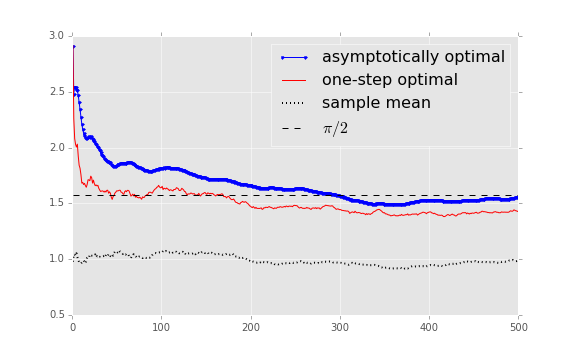
\includegraphics[scale=0.4]{one_bit_adpative}};
%\node[rotate = 90, scale = 0.7] at (-3.8,0) {$n \mathbb E \left({\theta}_n - \theta \right)^2$};
%\node[scale = 0.7] at (0,-2.4) {$n$};
%\end{tikzpicture}
\caption{Normalized empirical risk versus number of samples $n$ for $10,000$ Monte Carlo trials with $f(x)$ the standard normal density. In each trial, $\theta$ is chosen uniformly over the interval $(-1.64,1.64)$. The single interaction strategy uses $n_1 = \lfloor \sqrt{n} \rfloor$ samples for its first stage. 
\label{fig:adaptive_error}  }
\end{center}
\end{figure}
